\subsection{Descripción del filtro}
\label{sub:miniature_descripcion}

El filtro miniature es un caso particular de la familia de filtros por convolución, en los cuales se procesa una imagen realizando una convolución entre esta y una matriz determinada denominada \emph{kernel}. Las características del \emph{kernel} determinan el efecto resultante sobre la matriz; en este caso, el efecto logrado se conoce como desefoque gaussiano (se puede ver un ejemplo en la figura \ref{fig:filtro-miniature-ejemplo}), y se obtiene mediante el siguiente \emph{kernel}:

\[ \frac{1}{600} *  \left( \begin{array}{ccccc}
  1 &   5 &  18 &   5 &   1 \\
  5 &  32 &  64 &  32 &   5 \\
 18 &  64 & 100 &  64 &  18 \\
  5 &  32 &  64 &  32 &   5 \\
  1 &   5 &  18 &   5 &   1 \end{array} \right)\]

Operativamente, la imagen es procesada mediante una actualización pixel a píxel, reemplazando el valor de cada canal de color del pixel por una combinación lineal del valor de sus vecinos, cada uno ponderado por un coeficiente determinado por un elemento de la matriz. Se toma el elemento central del \emph{kernel} como coeficiente del pixel que se está procesando, y la posición relativa a los demás elementos de la matriz determina a cuál vecino corresponde en la combinación lineal. El factor $\frac{1}{600}$ es una constante de normalización que garantiza que el resultado sea un valor en el rango $[0, 255]$.

\begin{figure}[h]
\begin{center}
  
\includegraphics[scale=0.2]{secciones/filtro_miniature/imagenes/neo.jpg}
  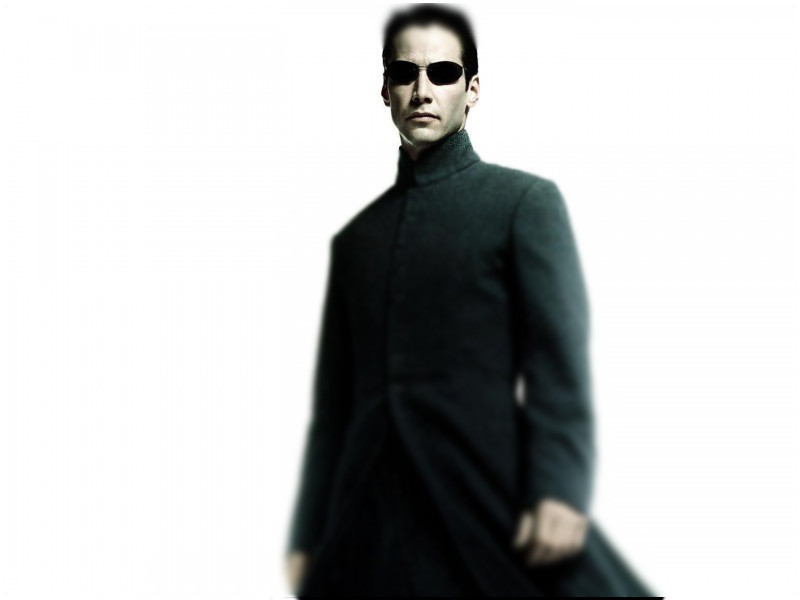
\includegraphics[scale=0.2]{secciones/filtro_miniature/imagenes/neo-miniature.jpg}
\end{center}
\caption{Imagen antes y después de aplicar el filtro miniature con parámetros de banda $0.08$ y $0.25$, y un total de 20 iteraciones.}
\label{fig:filtro-miniature-ejemplo}
\end{figure}

Se incorpora una leve modificación al modelo típico de filtro por convolución, limitando el efecto del filtrado a dos bandas dentro de la imagen; una banda superior, y una banda inferior, dejando la banda central de la imagen inalterada. Se especifican dos parámetros $0 < $ \param{topPlane} $<$ \param{bottomPlane} $ < 1$, de forma tal que las bandas quedan determinadas de esta forma:

\begin{center}
	\raggedright
	\hspace{100pt}\textbf{banda superior:} 	\hspace{10pt}filas 0 ... $topPlane * altura$\\
	\hspace{100pt}\textbf{banda media:} 		\hspace{22pt}filas $topPlane * altura + 1$ ... $bottomPlane * altura - 1$\\
	\hspace{100pt}\textbf{banda baja:} 		\hspace{31pt}filas $bottomPlane * altura$ ... $altura - 1$\\
\end{center}

Adicionalmente, se realizan múltiples iteraciones de filtrado, reduciendo el ancho de cada banda luego de cada iteración por:

\begin{center}
	\raggedright
	\hspace{100pt}$\Delta$\textbf{banda superior:} 	\hspace{10pt}$topPlane * altura / cantIteraciones$\\
	\hspace{100pt}$\Delta$\textbf{banda baja:} 		\hspace{31pt}$(1 - bottomPlane) * altura / cantIteraciones$\\
\end{center}

En el caso de los píxeles del borde, donde no existe el vecindario completo, se optó por exceptuarlos del filtrado, simplificando el procedimiento al saltear las dos primeras y dos últimas filas y columnas.

\subsection{Implementación en lenguaje C y lenguaje ensamblador}
\label{sub:miniature_implementaci_n_en_c}

El filtro se implementó en C mediante un ciclo que visita una vez por iteración a cada pixel de la banda superior y de la banda inferior, y actualizando el valor de sus tres canales de color por la combinación lineal descripta previamente.

Para este filtro, la implementación intuitiva en C resultó particularmente sugerente a la necesidad de buscar formas de optimizar el procedimiento, dado que cada pixel se lee de la memoria hasta 25 veces (una vez por cada vecino) resultando en un tiempo de ejecución prolongado. Además, el tipo de procesamiento realizado por cada pixel es el cómputo de una combinación lineal, para lo cual los procesadores utilizados están altamente optimizados. Realizar esta operación mediante un ciclo es un claro desperdicio de los beneficios brindados por el hardware.

\begin{figure}[h]
\begin{center}
  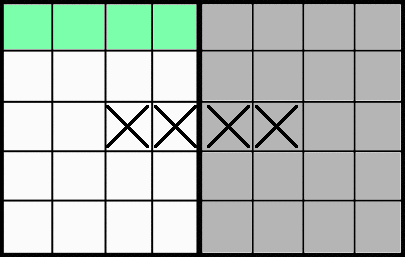
\includegraphics[scale=0.4]{secciones/filtro_miniature/imagenes/grid.png}
  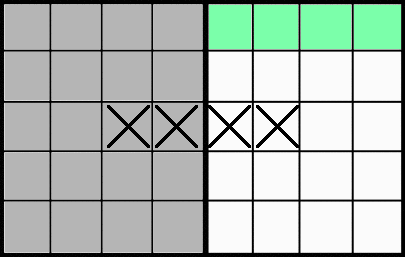
\includegraphics[scale=0.4]{secciones/filtro_miniature/imagenes/grid-inv.png}
\end{center}
\caption{Esquema de procesamiento filas izquierdas, filas derechas.}
\label{fig:filtro-miniature-grillas}
\end{figure}

Para implementar el mismo algoritmo en términos de procesamiento simultáneo, se trabajó con 4 píxeles por cada iteración del ciclo de convolución. Se procuró minimizar los accesos a memoria, mediante el esquema caracterizado por la figura (\ref{fig:filtro-miniature-grillas}): al procesarse los píxeles marcados con cruces, se leen previo al comienzo de la iteración los 20 píxeles sin sombrear. Se inicializan tres acumuladores, uno por cada canal de color, conteniendo la suma parcial \emph{sin normalizar} de los 4 pixeles en simultáneo. Esto es posible ya que el valor de la convolución para un determinado punto jamás excede el valor $255 * 600 = 153000$, el cual cabe en un entero \tipo{doubleword} y por lo tanto se pueden almacenar hasta 4 por registro XMM.

En los acumuladores se suma el aporte de cada uno de los 20 píxeles sin sombrear sobre cada uno de los 4 píxeles marcados con cruces, procesando fila por fila. Es decir, se toma la primer fila (de color verde en el diagrama), se calcula el aporte de cada uno de ellos sobre cada uno de los 4 píxeles con cruz, y se suma al acumulador. La operación se repite para cada uno de los tres canales, y para cada una de las 5 filas sin sombrear.

Para realizar este cálculo, se desempaquetan los tres canales de los píxeles en verde de forma tal de obtener máscaras del tipo:
$$[b_3, b_2, b_1, b_0, b_3, b_2, b_1, b_0]$$
$$[g_3, g_2, g_1, g_0, g_3, g_2, g_1, g_0]$$
$$[r_3, r_2, r_1, r_0, r_3, r_2, r_1, r_0]$$

y luego se realiza el producto interno con máscaras conteniendo elementos de la matriz con la siguiente forma:

$$[c_{30}, c_{20}, c_{10}, c_{00}, c_{31}, c_{21}, c_{11}, c_{01}]$$
$$[c_{32}, c_{22}, c_{12}, c_{02}, c_{33}, c_{23}, c_{13}, c_{03}]$$

donde $c_{ij}$ es el coeficiente del i-ésimo pixel verde sobre el j-ésimo pixel marcado con cruz.

El procesamiento simultáneo en esta etapa se limita a dos píxeles marcados con cruces por vez, ya que un producto del tipo $b_i * c_{ij}$ precisa de hasta un entero de tamaño \tipo{word}, permitiendo calcular hasta 8 productos por vez (y se requieren 4 productos por cada pixel marcado con cruz). Posteriormente, mediante sumas horizontales se obtienen 4 \tipo{doublewords} en un registro XMM, cada uno con una suma del tipo $b_3 * c_3 + b_2 * c_2 + b_1 * c_1 + b_0 * c_0$; este resultado luego se suma al acumulador (de azules, este caso). La operación se repite para cada canal, y para cada fila, obteniendo finalmente el aporte de los 20 píxeles sin sombrear, sobre los 4 píxeles marcados con cruces.

Como aclaración adicional, las máscaras con coeficientes utilizadas para realizar el producto se almacenan en forma de \tipo{bytes}, permitiendo reducir cuatro veces el tamaño requerido de haberse usado \tipo{floats}, y minimizando el costo de lectura.

El próximo paso consiste en leer de memoria los píxeles sobreados. Es importante notar que una vez leídas las filas de la derecha, ya se cuenta con todos los píxeles necesarios para terminar la acumulación sobre los 4 píxeles marcados con cruces; pero adicionalmente, \emph{las 4 filas de la derecha son reutilizadas para la acumulación de lado izquierdo en la próxima iteración}. Esto reduce significativamente la cantidad de lecturas a memoria en comparación a la implementación en C, y además mejora el uso de la memoria caché, ya que al leer los píxeles de lado izquierdo es muy probable que se acelere el acceso al bloque de píxeles del lado derecho.

Para finalizar la actualización, se realiza un proceso similar sobre las filas derechas, aunque es necesario espejar las máscaras de coeficientes utilizadas del lado izquierdo. La suma total luego se normaliza, y se empaqueta en el formato RGB para escribirse en la imagen destino.

La única salvedad o \emph{caso borde} resulta para los últimos 4 píxeles de cada fila, donde se escriben los píxeles del marco que se desea dejar inalterado. Sin embargo, la memoria pisada es válida (pertenece a la imagen), y es sencillo restaurarla realizando una copia desde la fuente; es decir, no hay que realizar retroceso en el puntero o lógica de borde.

\subsection{Comparación de performance}
\label{sub:comparaci_n_de_performance}

Se tomaron mediciones sobre ambas implementaciones con el criterio discutido en la sección de consideraciones generales, y se realizaron gráficos comparando la performance de la implementación en C y la implementación en lenguaje ensamblador.

\begin{figure}[H]
\begin{center}
  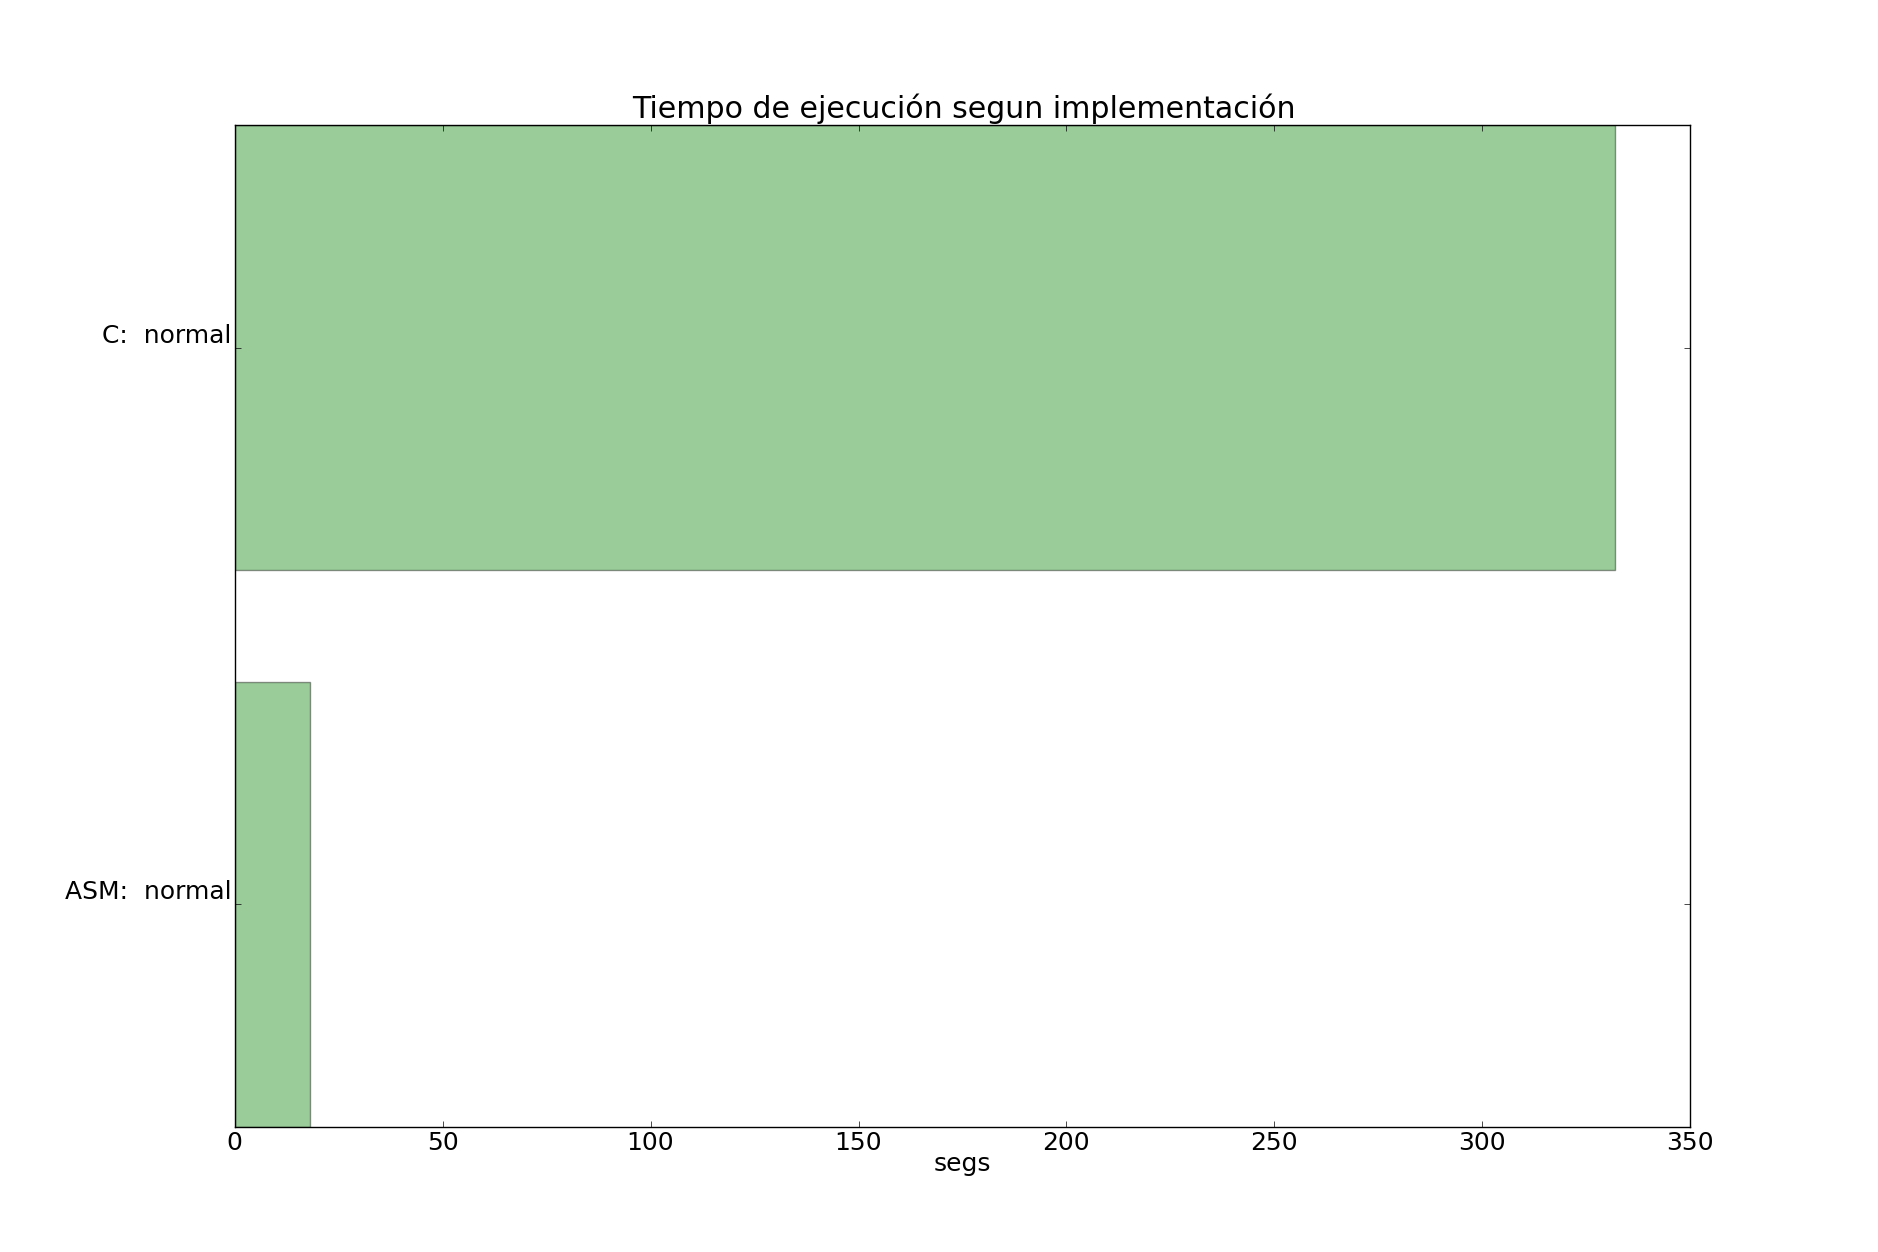
\includegraphics[scale=0.35]{secciones/filtro_miniature/graficos/C_ASM_perf.png}
  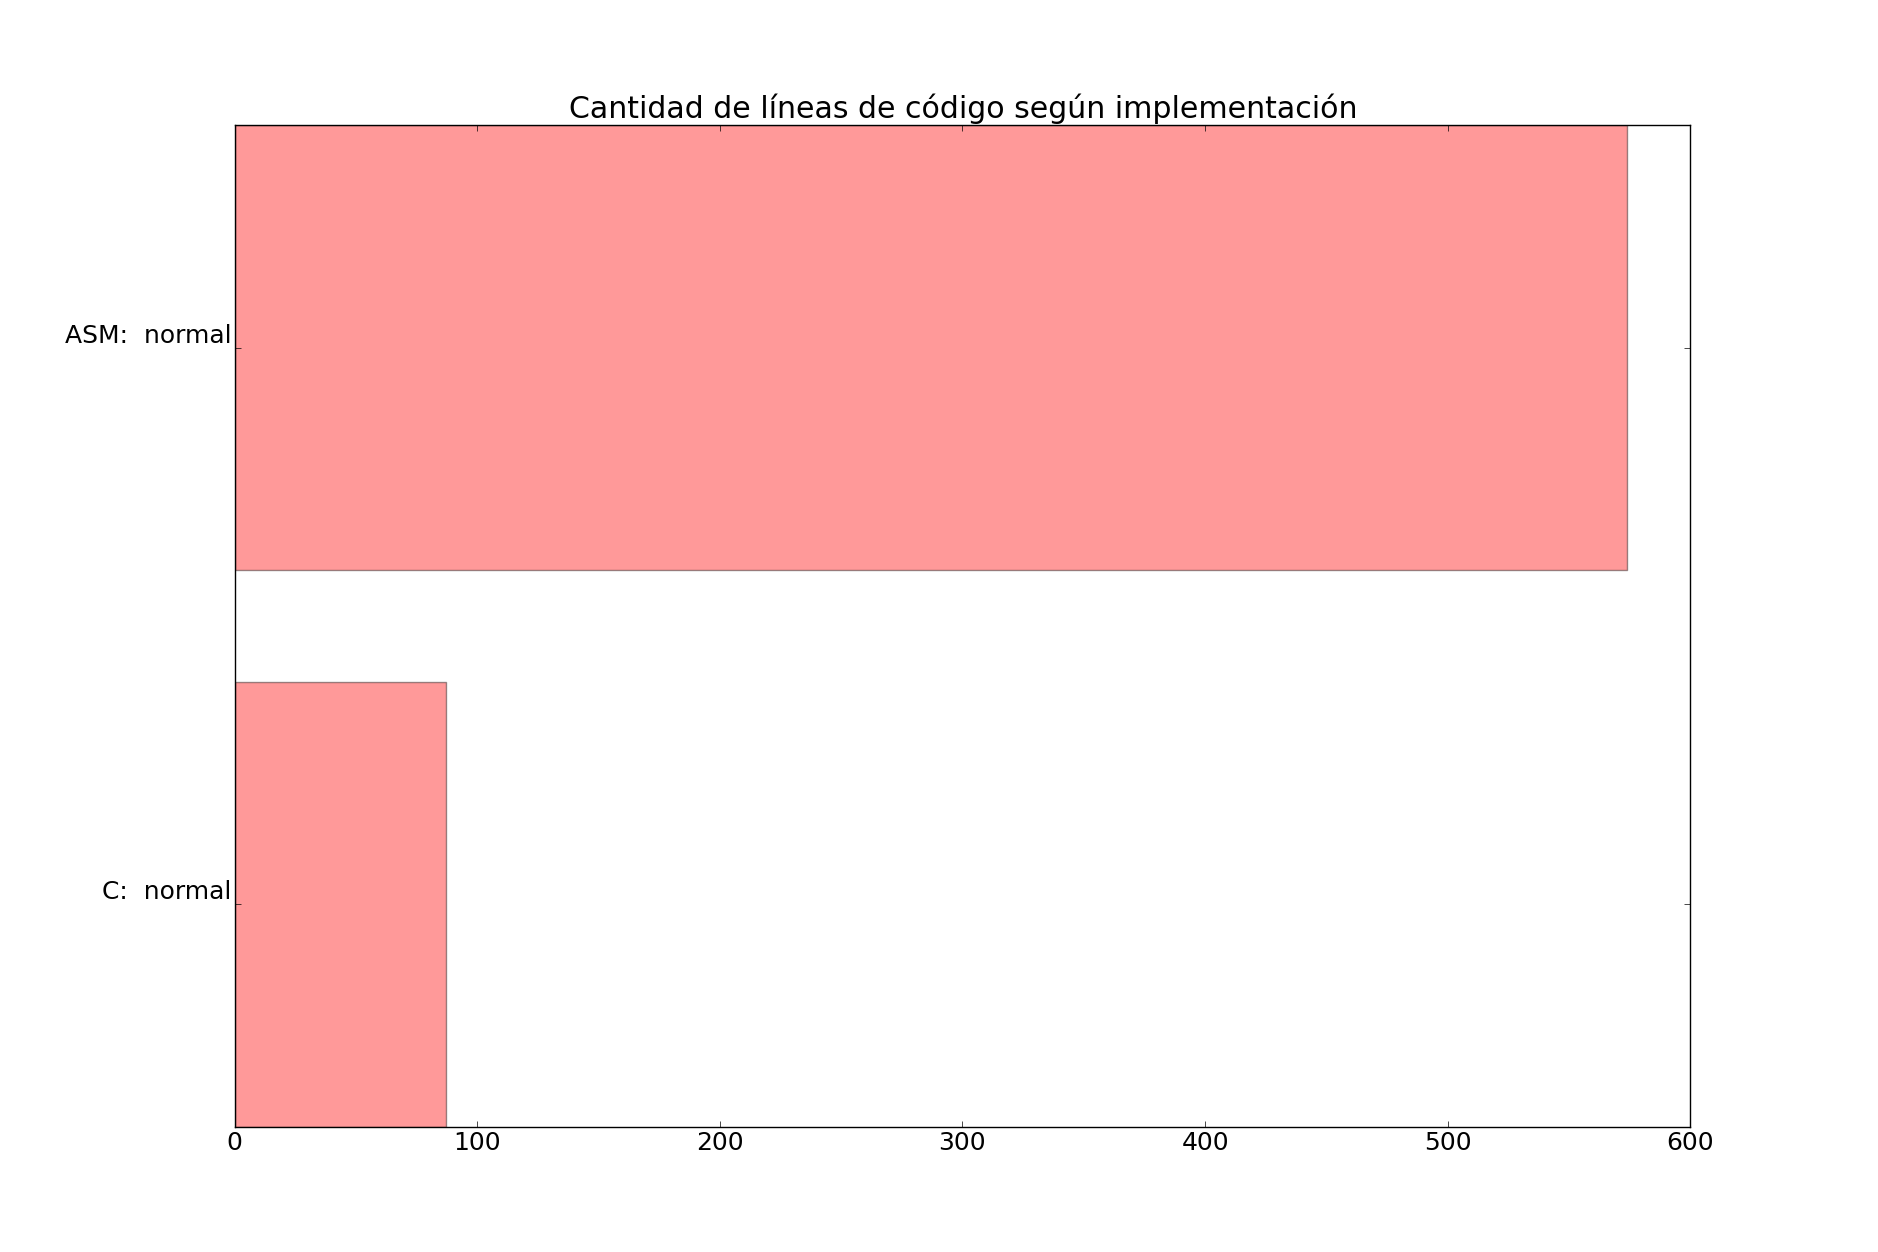
\includegraphics[scale=0.35]{secciones/filtro_miniature/graficos/C_ASM_loc.png}
\end{center}
\caption{Comparación de performance (superior) y cantidad de líneas de código (inferior) entre versión C básica y versión ASM básica.}
\label{fig:filtro-miniature-C-vs-ASM}
\end{figure}

En el caso del filtro miniature, la diferencia de performance entre la versión C y la versión ASM es incluso más radical que para el filtro de color, con mejoras de entre \textbf{x18} y \textbf{x20} veces. La proporción en cantidad de líneas de código, sin embargo, es similar (alrededor de 6 veces). Esto revela que el código C en su versión más intuitiva es particularmente subóptimo para este tipo de procesamiento, dictando que el procesamiento simultáneo y la utilización de los recursos del hardware son fundamentales para cualquier implementación performante de un filtro de convolución.

\subsection{Profiling para la implementación en ASM}
\label{sub:profiling_para_la_implementaci_n_en_asm}

Para estudiar cuáles son los puntos de la implementación en lenguaje ensamblador que es necesario optimizar para mejorar la performance, se realizaron dos mediciones adicionales sobre el código, incluyendo dos variantes:

\begin{itemize}
	\item Todos los movimientos de lectura/escritura a memoria removidos
	\item La lógica de flujo intácta, pero sin realizar la acumulación por filas descripta previamente durante el ciclo de procesamiento.
\end{itemize}

No fue posible medir dentro de la misma ejecución las diferentes partes del código, ya que cualquier mecanismo de medición incluye una costo en clocks que se vuelve significativo si se introduce dentro del ciclo principal. Por lo tanto, se midió el tiempo total de 3 ejecuciones con el código en sus tres variantes. Se incluye en la figura \ref{fig:filtro-miniature-ASM-profiling} un gráfico de circular que \textbf{no} debe interpretarse como el porcentaje de tiempo insumido por cada una de las partes medidas (procesamiento vs lectura/escritura), ya que fueron medidas por separado y sin dudas influyen una en la otra (debido a la ejecución fuera de orden que realiza el procesador). Sin embargo, sí se puede interpretar como el porcentaje de tiempo insumido por cada versión en el total de las 3 ejecuciones, permitiendo estimar una relación entre el costo de las distintas partes.

\begin{figure}[H]
\begin{center}
  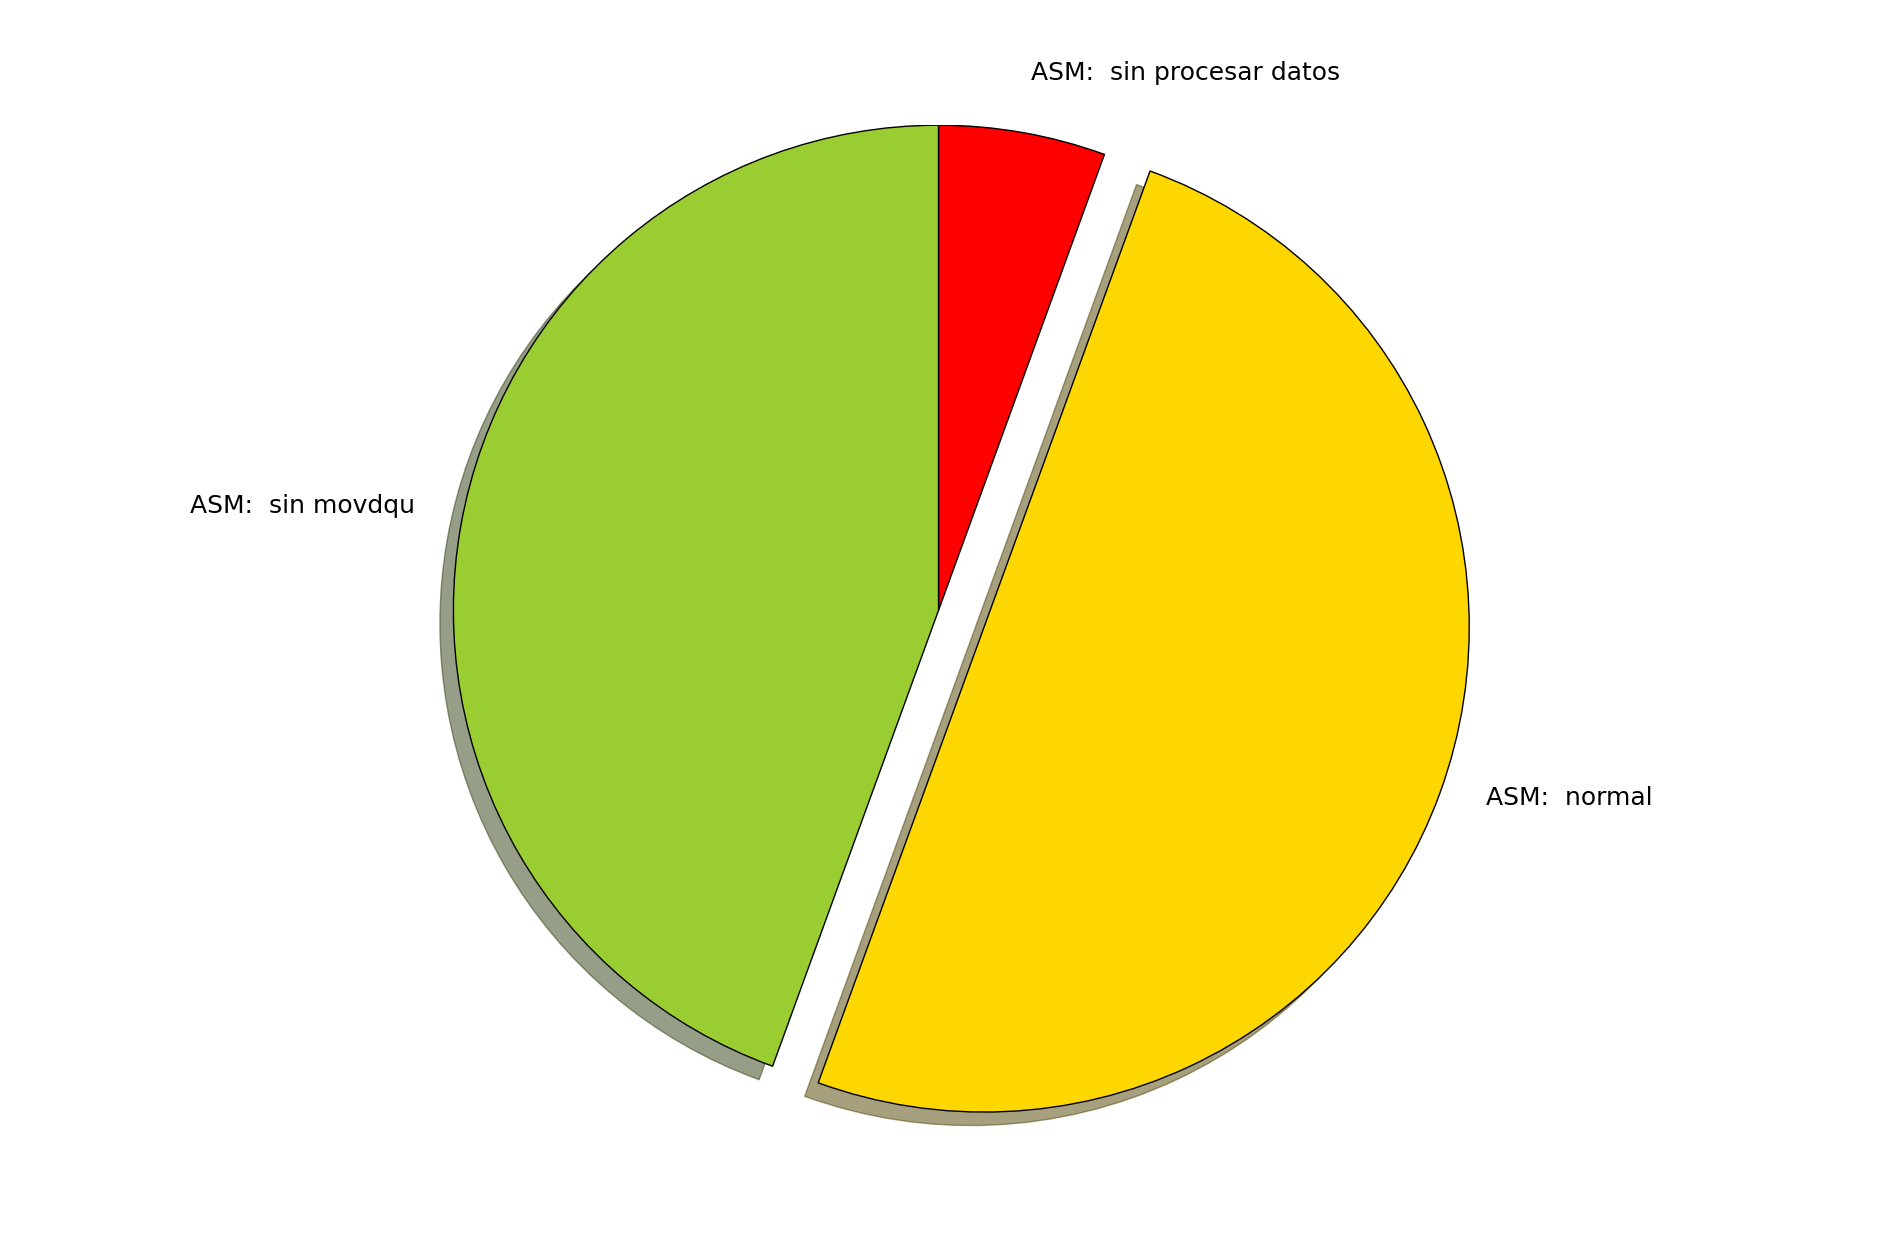
\includegraphics[scale=0.35]{secciones/filtro_miniature/graficos/ASM_normal_sinmovdqu_sinprocesardatos.png}
\end{center}
\caption{Gráfico circular mostrando el porcentaje de tiempo insumido por tres versiones del código ASM: completo, sin lectura/escritura, sin procesamiento.}
\label{fig:filtro-miniature-ASM-profiling}
\end{figure}

Se puede observar en el gráfico que la instancia del programa sin realizar el procesamiento de los píxeles leídos fue signficativamente más veloz que las demás; es decir, la mayor parte del costo total deviene de la etapa de procesamiento. Esta información fue inesperada, ya que la implementación se hizo con una fuerte consideración en evitar las lecturas a memoria, posiblemente incurriendo en costo de procesamiento adicional para evitarlas. Esto indica que un próximo paso en la optimización sería reducir el costo de procesamiento mediante la relajación de la restricción en las lecturas a memoria (posiblemente haciendo uso de mayor número de máscaras, lo cual se evitó por la falta de registros XMM disponibles).